\documentclass[11pt,a4paper]{article}
\usepackage[a4paper,margin=2.3cm]{geometry}
\usepackage{graphicx}
\usepackage{array}
\usepackage{longtable}
\usepackage{url}
\usepackage[T1]{fontenc}
\usepackage{lmodern}
\usepackage{xeCJK}
\usepackage{hyperref}
\hypersetup{colorlinks=true,linkcolor=blue,citecolor=blue,urlcolor=blue}
\graphicspath{{figures/}{../figures/}}
\setCJKmainfont{SimSun}
\setlength{\parindent}{2em}
\setlength{\parskip}{0.35em}
\setlength{\tabcolsep}{4pt}
\emergencystretch=1em
\newcommand{\code}[1]{\texttt{#1}}
\newcommand{\barunit}{\,bar}
\newcommand{\toprule}{\hline}
\newcommand{\midrule}{\hline}
\newcommand{\bottomrule}{\hline}
\newcommand{\hashblock}{%
\begin{center}
\begingroup\ttfamily\small
24128AAD2EE45EEA7E6B63EBBD9992CD\\
F25D0483A2CEBEFBFC13BC69079AF1F2
\endgroup
\end{center}}

\title{How Split Protocols Change Reported Performance on a Public Hydraulic Test Rig: An Audit of Accumulator-Level Identification and Nominal-Pressure Error}
\author{Chen-Yu Yan}
\date{October 2026}

\begin{document}
\maketitle

\begin{abstract}
\sloppy
\textbf{Objective:} To evaluate how data-splitting protocols change reported accumulator pressure-level identification on a public hydraulic test rig, and to compare discrete target representation with numeric regression for nominal-pressure error.

\textbf{Methods:} We used the UCI Condition Monitoring of Hydraulic Systems dataset, which contains 2,205 60-s cycles and 17 signal channels. Seventy cycle-level summary features were extracted from six pressure channels and one motor-power channel. The main task was classification of four nominal accumulator pressure levels (90, 100, 115, and 130~bar). Four outer protocols were compared: random cycles, profile-contiguous blocks, observed four-component combination holdout (state4-OC), and five-label combinations including the stable flag (state5). Nested grouped cross-validation used five split seeds, with model selection inside each outer training set. Fixed-model and paired classification--regression audits used the same state4-OC outer folds.

\textbf{Results:} Across five seeds, median pooled OOF balanced accuracy was 0.983 (0.981--0.985) for random cycles and 0.870 (0.860--0.875) for state4-OC. On the same state4-OC OOF cycles, MAE after mapping classification labels to nominal pressure values was 1.83~bar, compared with 7.74~bar for numeric regression. The weighting audit gave classification accuracies of 0.884, 0.876, and 0.866 for cycle, state4-combination, and profile-block weighting, respectively; regression MAE was 7.74, 5.35, and 5.39~bar.

\textbf{Conclusion:} In this dataset and workflow, the split protocol changes both the point estimate and the estimand. The differences are properties of the full evaluation workflow, not an identified causal leakage amount. The four nominal levels support a discrete state-identification evaluation and provide no evidence for continuous-pressure or cross-device performance. The contribution is a reproducible evaluation that links split protocol, estimand, and error representation.
\end{abstract}

\noindent\textbf{Keywords:} hydraulic system; condition monitoring; cross-validation; grouped evaluation; accumulator pressure; ordinal error

\section{Introduction}
Reported performance in hydraulic condition monitoring depends on how observations are split as well as on the features and classifier. We use the UCI Condition Monitoring of Hydraulic Systems dataset, which records multirate signals and component-state profiles from one hydraulic test rig. The official page reports 2,205 instances, 17 signal files, DOI 10.24432/C5CW21, and a CC BY 4.0 licence~\cite{uci}. Prior work has studied this system with multivariate statistics, sensor-fault compensation, and cycle-level feature extraction~\cite{helwigstats,helwigfault,schneider}; Chinese studies provide complementary task references for multi-component identification, multisensor health assessment, and deep-model diagnosis~\cite{zhou,zhaoxu,shan,zheng}.

Several studies already classify multiple components in this dataset or analyse sensor attribution~\cite{yildirim,konig}. Zhan and Liu~\cite{zhan} report a high test accuracy for a 144-state task, but do not fully specify the train/test proportion, split unit, or normalization-fitting scope. A 2026 preprint uses block-disjoint evaluation and blockwise joint conformal prediction~\cite{bui}. These studies show that the dataset can produce high classification scores and that the scores should be read together with the split unit, target definition, and uncertainty report. The present study therefore focuses on the evaluation protocol: what estimand each split approximates, and whether discrete pressure labels and numeric regression lead to the same error interpretation.

Repeated cycles from one rig make the split itself part of the question. Random-cycle splitting asks whether a new cycle can be recognized under similar observed conditions; profile-contiguous blocks or component-state holdouts change the structure being withheld. Cross-validation research likewise recommends matching the split to the prediction scenario~\cite{roberts}. The resulting scores are therefore treated as results for different evaluation scenarios rather than as simple high and low estimates of one parameter.

The study asks how cycle, profile-contiguous-block, and component-state splits change the accumulator-level classification point estimate under fixed cycle-level features and a candidate-model workflow, and what nominal-pressure errors arise when discrete classification and numeric regression are paired on the same state4-OC held-out cycles. The contribution is a reproducible protocol--estimand mapping that combines multi-seed OOF results, weighting audits, and same-cycle error comparisons. The five-seed, fixed-model, and paired-error analyses were added during the audit and are reported as supplementary sensitivity analyses.

\section{Materials and methods}

\subsection{Data source and structural audit}

We used the official UCI compressed archive of the Condition Monitoring of Hydraulic Systems dataset~\cite{uci}. The local archive has the following SHA-256 hash:\hashblock It contains 2,205 consecutively numbered 60-s cycles, 17 signal files, and one five-column profile per cycle. Pressure signals PS1--PS6 and motor power EPS1 are sampled at 100~Hz with 6,000 points per cycle. Flow signals FS1 and FS2 are sampled at 10~Hz with 600 points per cycle. Temperature TS1--TS4, vibration VS1, CE, CP, and SE are sampled at 1~Hz with 60 points per cycle.

The local audit checked, line by line, row counts, points per cycle, blank rows, parsing failures, non-finite values, and profile alignment in all 17 signal files. Each file contains 2,205 cycles with the points per cycle stated in the official documentation; no blank rows, parsing failures, or non-finite values were found. This audit establishes file structure and numerical parsability. Sensor calibration, measurement bias, and independence of experimental batches require external verification.

The first four profile columns describe cooler, valve, internal pump leakage, and accumulator states; the last column is the stable flag. Cooler levels are 3, 20, and 100; valve levels are 73, 80, 90, and 100; pump leakage has levels 0, 1, and 2; and accumulator labels are 90, 100, 115, and 130~bar. A stable value of 0 denotes that the stable condition was reached, whereas 1 indicates that static conditions may not yet have been reached. We treat this as a condition flag rather than a fifth fault class. CE and CP are marked as virtual signals in the data documentation, and SE is defined as an efficiency factor; we do not infer that the three represent independent physical sensors~\cite{uci}.

\subsection{Tasks and analysis unit}

The primary task is four-level accumulator-state classification. Pump internal leakage classification is a supplementary task. The basic unit is one complete 60-s cycle; 2,205 cycles are not treated as 2,205 independent experiments. To avoid interpreting the grouping as formal time or batch holdout, we call adjacent cycles with exactly identical five-column profiles ``profile-contiguous blocks.'' There are 194 blocks: 36 of length one cycle, 154 of length ten, one of length 19, two of length 200, and one of length 210. Ignoring stable, there are 144 distinct four-component state combinations; including stable, there are 180 distinct five-column state vectors. Profile blocks and state combinations are derived from the public profile and are not official batch or equipment identifiers.
To prevent this protocol from being read as equipment or batch validation, we call the exact four-column profile combination holdout the ``observed four-component combination holdout (\code{state4-OC}; OC = observed-combination). ``Unseen means only that an exact combination code is absent from the training fold; the same pressure levels remain present in other combinations from the same rig and recorded dataset. The name does not imply unseen equipment, accumulator levels, independent acquisition batches, or field operation. The raw scripts and result files retain \code{state4} as an implementation identifier.

\subsection{Feature construction}

The main classifier uses the \code{pressure\_power} channel group: PS1--PS6 and EPS1, seven 100-Hz measurement channels. For each signal and cycle we computed the mean, population standard deviation (ddof=0), minimum, maximum, range, 10th percentile, median, 90th percentile, last-minus-first value, and the mean absolute difference between adjacent samples. Percentiles use NumPy's default linear interpolation in \code{quantile}. Ten features per signal yield 70 features. We call last-minus-first a difference feature and the mean adjacent absolute difference a change feature; neither is interpreted as a physical slope or rate. Features are computed independently for each 60-s cycle. Cycle order is used only to construct profile-contiguous blocks and state groups and is not an input to the model.

\subsection{Classifiers and nested model selection}

Candidate classifiers are logistic regression, an RBF-kernel support-vector machine (RBF-SVM), and a random forest. Logistic regression and the SVM use a \code{StandardScaler} fitted inside the training fold; the random forest is not standardized. Candidate model and parameter are selected in each outer training fold by balanced accuracy. The search space is logistic-regression $C\in\{0.1,1,10\}$ with maximum 2,500 iterations; RBF-SVM $C\in\{1,10\}$ with \code{gamma=``scale''}; and a random forest with 300 trees and \code{max\_features=``sqrt''}. The six resulting configurations are used for every protocol.

The main analysis uses five outer folds and three inner folds in nested cross-validation, reducing the selection bias that arises when a candidate is selected and evaluated on the same cross-validation error~\cite{varma}. Each outer test fold is predicted by a model selected and fitted using only the remaining training data. Both outer and inner classification splits use \code{StratifiedGroupKFold} with \code{shuffle=True}; for seed $s$, inner-fold seed $s+k$ is used for the $k$th outer fold. Under the random protocol, each cycle is assigned a unique group, so class stratification is retained while nearby cycles can be distributed across training and test sets. The other protocols use the predefined profile-contiguous, state4-OC, or state5 group identifiers.

The five-seed analysis uses seeds \code{20261013} through \code{20261017}. Seed 20261013 is the original main run; the other four seeds were added after inspecting that run to assess split sensitivity and stability and are not preregistered repeated experiments. The internal random seed of the classifiers, including the random forest, is fixed at \code{random\_state=20261013}; seed variation therefore changes the cross-validation partition but not the forest's internal draw. The software environment is Python 3.14.3, NumPy 2.4.4, SciPy 1.17.1, and scikit-learn 1.9.1.
\par
These five seeds are not five independent experiments or repeated samples from a target population; their range describes reallocation of the same 2,205 physical cycles. Because the additional four seeds were decided after inspecting the 20261013 result, analysis-selection risk remains. Re-running the same cycles cannot remove that risk, so the seed range is not an independent robustness confirmation, a confidence interval, or significance evidence.

For seed 20261013 and the same outer folds, we additionally fitted three fixed configurations without inner selection: logistic regression with $C=10$, RBF-SVM with $C=10$, and a 300-tree random forest. This separates changes due to model selection from protocol differences under fixed models. It was added after examining the nested results and is an exploratory comparison.

\subsection{Numeric-regression comparison}

The auxiliary regression task uses 90, 100, 115, and 130 as numeric responses. Candidates are Ridge regression with $\alpha\in\{0.1,1,10,100\}$, RBF-SVR with $C\in\{1,10,100\}$, \code{gamma=``scale''}, and $\epsilon=0.1$, and a 300-tree random-forest regressor with \code{max\_features=``sqrt''}. Linear and support-vector models are standardized inside the training fold. The regression candidate is selected by inner-fold mean absolute error (MAE), and outer and inner splits use the same state4-OC stratified grouped folds. Numeric predictions are not constrained to 90--130~bar.

For a directly readable level baseline, classifier OOF categories are mapped to their nominal pressure values (90, 100, 115, or 130~bar) and paired with regression predictions by the same cycle ID, true label, and outer fold. This mapping is a post hoc derived comparison from the existing classifier OOF predictions; the classifier was selected by balanced accuracy rather than pressure MAE. The labels are four discrete set points rather than continuously measured pressure truth. The bar error of the classification mapping therefore expresses deviation from a nominal level; continuous pressure measurement requires a continuous reference and independent acquisition batches.

\subsection{Supplementary analyses}

Supplementary pump-leakage classification follows the main \code{pressure\_power} features, state4-OC grouping, seed 20261013, five outer and three inner folds, nested candidate-model selection, and balanced-accuracy criterion. It is an exploratory check of another component label in the same dataset.

Accumulator channel-group sensitivity compares five sets under the same state4-OC split and seed: \code{all} contains all 17 signals (170 features); \code{physical} contains 14 signals excluding CE, CP, and SE (140 features); \code{low\_rate} contains TS1--TS4, VS1, CE, CP, and SE (80 features); \code{pressure\_flow} contains PS1--PS6, FS1, and FS2 (80 features); and \code{pressure\_power} contains PS1--PS6 and EPS1 (70 features). Each group uses the same nested selection workflow. This comparison evaluates predictive results for existing channel groupings and does not establish hardware configuration, sensor cost, or deployment benefit.

Stable-stratified results are calculated from the complete state4-OC OOF table by stable flag without refitting within each stratum. The common-support description is limited to state4-OC combinations containing both stable=0 and stable=1 cycles, and reports their cycle counts and accumulator-label composition. No equal-weight paired effect is estimated across combinations. These are conditional descriptions; differing sample sizes and level composition preclude a causal interpretation of stable status.

\subsection{Split protocols and estimands}

The four split protocols are defined in Table~\ref{tab:protocols}.

\begin{table}[htbp]
\centering\small
\caption{Split protocols, intended scenarios, and known limits.}
\label{tab:protocols}
\begin{tabular}{p{0.18\linewidth}p{0.22\linewidth}p{0.29\linewidth}p{0.24\linewidth}}
\toprule
Protocol & Group unit & Main test scenario & Known limitation\\
\midrule
random & Individual cycle & Randomly hold out cycles from the same recorded population & Adjacent or repeated conditions may cross train/test sets\\
profile-contiguous block & Adjacent cycles with identical five-column profiles & Hold out contiguous constant-state blocks derived from profiles & Strongly unequal block lengths; neighboring time blocks can still be split; not formal batch holdout\\
state4-OC & Exact cooler--valve--pump-leak--accumulator combination & Hold out an unseen observed four-component combination while pressure levels occur in other combinations & Not a test of unknown pressure levels, equipment, batches, or field operation\\
state5 & Exact four-component state plus stable flag & Hold out an observed five-label combination & Does not ensure isolation of adjacent or otherwise correlated time periods\\
\bottomrule
\end{tabular}
\end{table}

To bind metric interpretation to scenarios that can be approximated from the public profile, we use Table~\ref{tab:decision}. ``Deployment target'' here means an evaluation scenario approximated by the profile and is not field validation.

\begin{table}[htbp]
\centering\small
\caption{Evaluation scenarios and extrapolations not supported by the present data.}
\label{tab:decision}
\begin{tabular}{p{0.24\linewidth}p{0.16\linewidth}p{0.25\linewidth}p{0.27\linewidth}}
\toprule
Approximate evaluation target & Candidate protocol & Estimand & Extrapolation not supported\\
\midrule
New cycles on the same rig under observed states & random & Cycle-level point prediction & Generalization to unknown equipment, batch, or time period\\
Unseen observed four-component combinations on the same rig & state4-OC & Cycle-level point prediction under component-combination holdout & Unknown accumulator levels, independent equipment, or industrial sites\\
Holdout of adjacent identical-profile segments & profile-contiguous block & Point prediction under profile-derived block holdout & Formal time batches, acquisition dates, or causal time effects\\
Discrimination of observed stable-condition combinations & state5 & Point prediction under five-label-combination holdout & Causal effect of stable status or equipment independence\\
\bottomrule
\end{tabular}
\end{table}

Cooler labels have temporal ordering, while the dataset has no usable equipment identifier, independent acquisition date, or formal batch identifier. Thus each grouping prevents a specified observed unit from crossing folds; statistical independence of cross-fold samples still requires equipment or batch information. All four protocols change the training/test composition, shareable state information, and model-selection environment. Their differences are differences between evaluation workflows and do not identify an amount of data leakage or a causal effect of splitting.

\subsection{Metrics and aggregation}

The primary classification results report accuracy, balanced accuracy, macro F1, and a confusion matrix. Accuracy weights cycles equally. Balanced accuracy is the arithmetic mean of class recalls, and macro F1 is the arithmetic mean of class-level F1 scores. For pooled OOF metrics, predictions from all outer test folds are first concatenated and then evaluated; balanced accuracy and macro F1 therefore average classes equally on the cycle-level OOF table. Group-level majority-vote accuracy first takes the mode of true and predicted labels within each group and then averages groups equally.

Ordinal error is computed from the index of the four levels [90, 100, 115, 130]. We report exact-level accuracy, one-neighbour hit rate (index distance $\leq 1$, including exact hits), mean level distance, and counts at distances 0, 1, 2, and 3. Numeric regression additionally reports MAE, RMSE, and $R^2$ in raw bar units. In addition to cycle-pooled estimands, we first compute cycle loss within each state4-OC combination or profile-contiguous block and then average units equally; MAE is also averaged equally over the four true pressure levels. These are distinct estimands, and their unit-level descriptive intervals are not confidence intervals for devices or batches. For the five split seeds, pooled OOF metrics are summarized by median, range, mean, and standard deviation; the main tables show median and range. These ranges describe reallocation of folds for the same dataset and are not population confidence intervals. We do not test folds or seeds for significance because training sets overlap and the same physical cycles are reused across seeds.

\section{Results}

\subsection{Data and group structure}

The structural audit confirmed complete alignment of 2,205 cycles and 17 signal files. Accumulator labels 90, 100, 115, and 130~bar occur in 808, 399, 399, and 599 cycles, respectively. Stable=0 and stable=1 occur in 1,449 and 756 cycles. The grouping registry contains 194 profile-contiguous blocks and 144 four-component state combinations. Block lengths are markedly unequal: two blocks of 200 cycles, one of 210 cycles, and one of 19 cycles dominate the long segments. Profile-block holdout is therefore constrained by a small number of long blocks and by temporal ordering.

\subsection{Protocol sensitivity with nested model selection}

Table~\ref{tab:main} summarizes pooled OOF balanced accuracy and macro F1 for the five split seeds. The five-seed median and range are the primary estimate; the original single seed is reference only. Random-cycle splitting exceeded state4-OC for all five seeds, whereas the ordering among profile blocks, state4-OC, and state5 was not stable. Median balanced accuracy was 0.983 for random cycles and 0.870 for state4-OC, with ranges 0.981--0.985 and 0.860--0.875. The paired random-minus-state4-OC balanced-accuracy difference had median 0.111 (0.107--0.124), macro-F1 difference 0.116 (0.110--0.124), and accuracy difference 0.100 (0.093--0.105). These differences describe changes in fold allocation for the same cycles; no significance test is performed. For the original seed 20261013, balanced accuracy was 0.981, 0.882, 0.870, and 0.875 for random, profile-contiguous block, state4-OC, and state5, respectively; the corresponding macro-F1 values were 0.982, 0.880, 0.866, and 0.872. Because the additional four seeds were added after inspecting the initial result, they cannot be interpreted as independent robustness confirmation, confidence intervals, or significance evidence.

\begin{table}[htbp]
\centering\small
\caption{Pooled OOF results across five split seeds. Values are medians with the five-seed range in parentheses.}
\label{tab:main}
\begin{tabular}{lcc}
\toprule
Protocol & Balanced accuracy & Macro F1\\
\midrule
Random cycles & 0.983 (0.981--0.985) & 0.982 (0.981--0.985)\\
Profile-contiguous blocks & 0.880 (0.873--0.887) & 0.878 (0.872--0.885)\\
State4-OC four-component combinations & 0.870 (0.860--0.875) & 0.866 (0.859--0.872)\\
State5 five-label combinations & 0.876 (0.871--0.891) & 0.872 (0.868--0.889)\\
\bottomrule
\end{tabular}
\end{table}

The random-cycle and state4-OC balanced-accuracy ranges do not overlap across the five seeds. This describes stability of alternative partitions of the same physical cycles, not independent replications or a significance test. The higher random-split score is compatible with similar or repeated operating-condition information crossing folds, but this design cannot assign the difference solely to leakage. The four additional seeds were chosen after inspecting the original result and therefore remain post hoc sensitivity analysis.

A weighting audit further separated cycle-pooled and unit-equal estimands. Cycle-weighted classification accuracy was 0.884; averaging within each of 144 state4-OC combinations and then weighting combinations equally gave 0.876, while the analogous 194-block estimate was 0.866. Numeric-regression MAE was 7.741, 5.346, and 5.390~bar for cycle, state4-OC-combination, and profile-block weighting, respectively; pressure-level-equal MAE was 6.850~bar. The regression result is therefore materially weight-sensitive. The full fold distribution and unit-level audit are in \code{results/weighted\_metrics\_audit\_20261016.json}.

\subsection{Protocol comparison under fixed models}

The supplementary fixed-classifier analysis shows that the size of the protocol difference depends on the classifier (Table~\ref{tab:fixed}). Random-forest balanced accuracy is 0.981 under random cycles and 0.760, 0.744, and 0.766 under profile blocks, state4-OC, and state5. RBF-SVM balanced accuracy is 0.920 for random cycles and about 0.720--0.736 under the three grouped protocols. Logistic-regression performance is 0.930 for random cycles and 0.870--0.882 for the grouped protocols. In the main nested search, random-protocol folds all selected the random forest, whereas state4-OC folds all selected logistic regression with $C=10$. The main random-versus-state4-OC difference therefore includes a change in model selection. Fixed-model results show that model sensitivity is not uniform, so the main difference cannot be interpreted as a classifier-independent split effect.

\begin{table}[htbp]
\centering\small
\caption{Fixed-classifier pooled OOF balanced accuracy for seed 20261013.}
\label{tab:fixed}
\begin{tabular}{lcccc}
\toprule
Fixed model & Random & Profile block & State4-OC & State5\\
\midrule
Logistic regression, $C=10$ & 0.930 & 0.882 & 0.870 & 0.875\\
RBF-SVM, $C=10$ & 0.920 & 0.736 & 0.720 & 0.729\\
Random forest, 300 trees & 0.981 & 0.760 & 0.744 & 0.766\\
\bottomrule
\end{tabular}
\end{table}

Table~\ref{tab:fixed} is an exploratory reference from the original seed. The fixed-model comparison was added after examining the main results, and the protocols still differ in test composition and train/test dependence.

\begin{figure}[htbp]
\centering
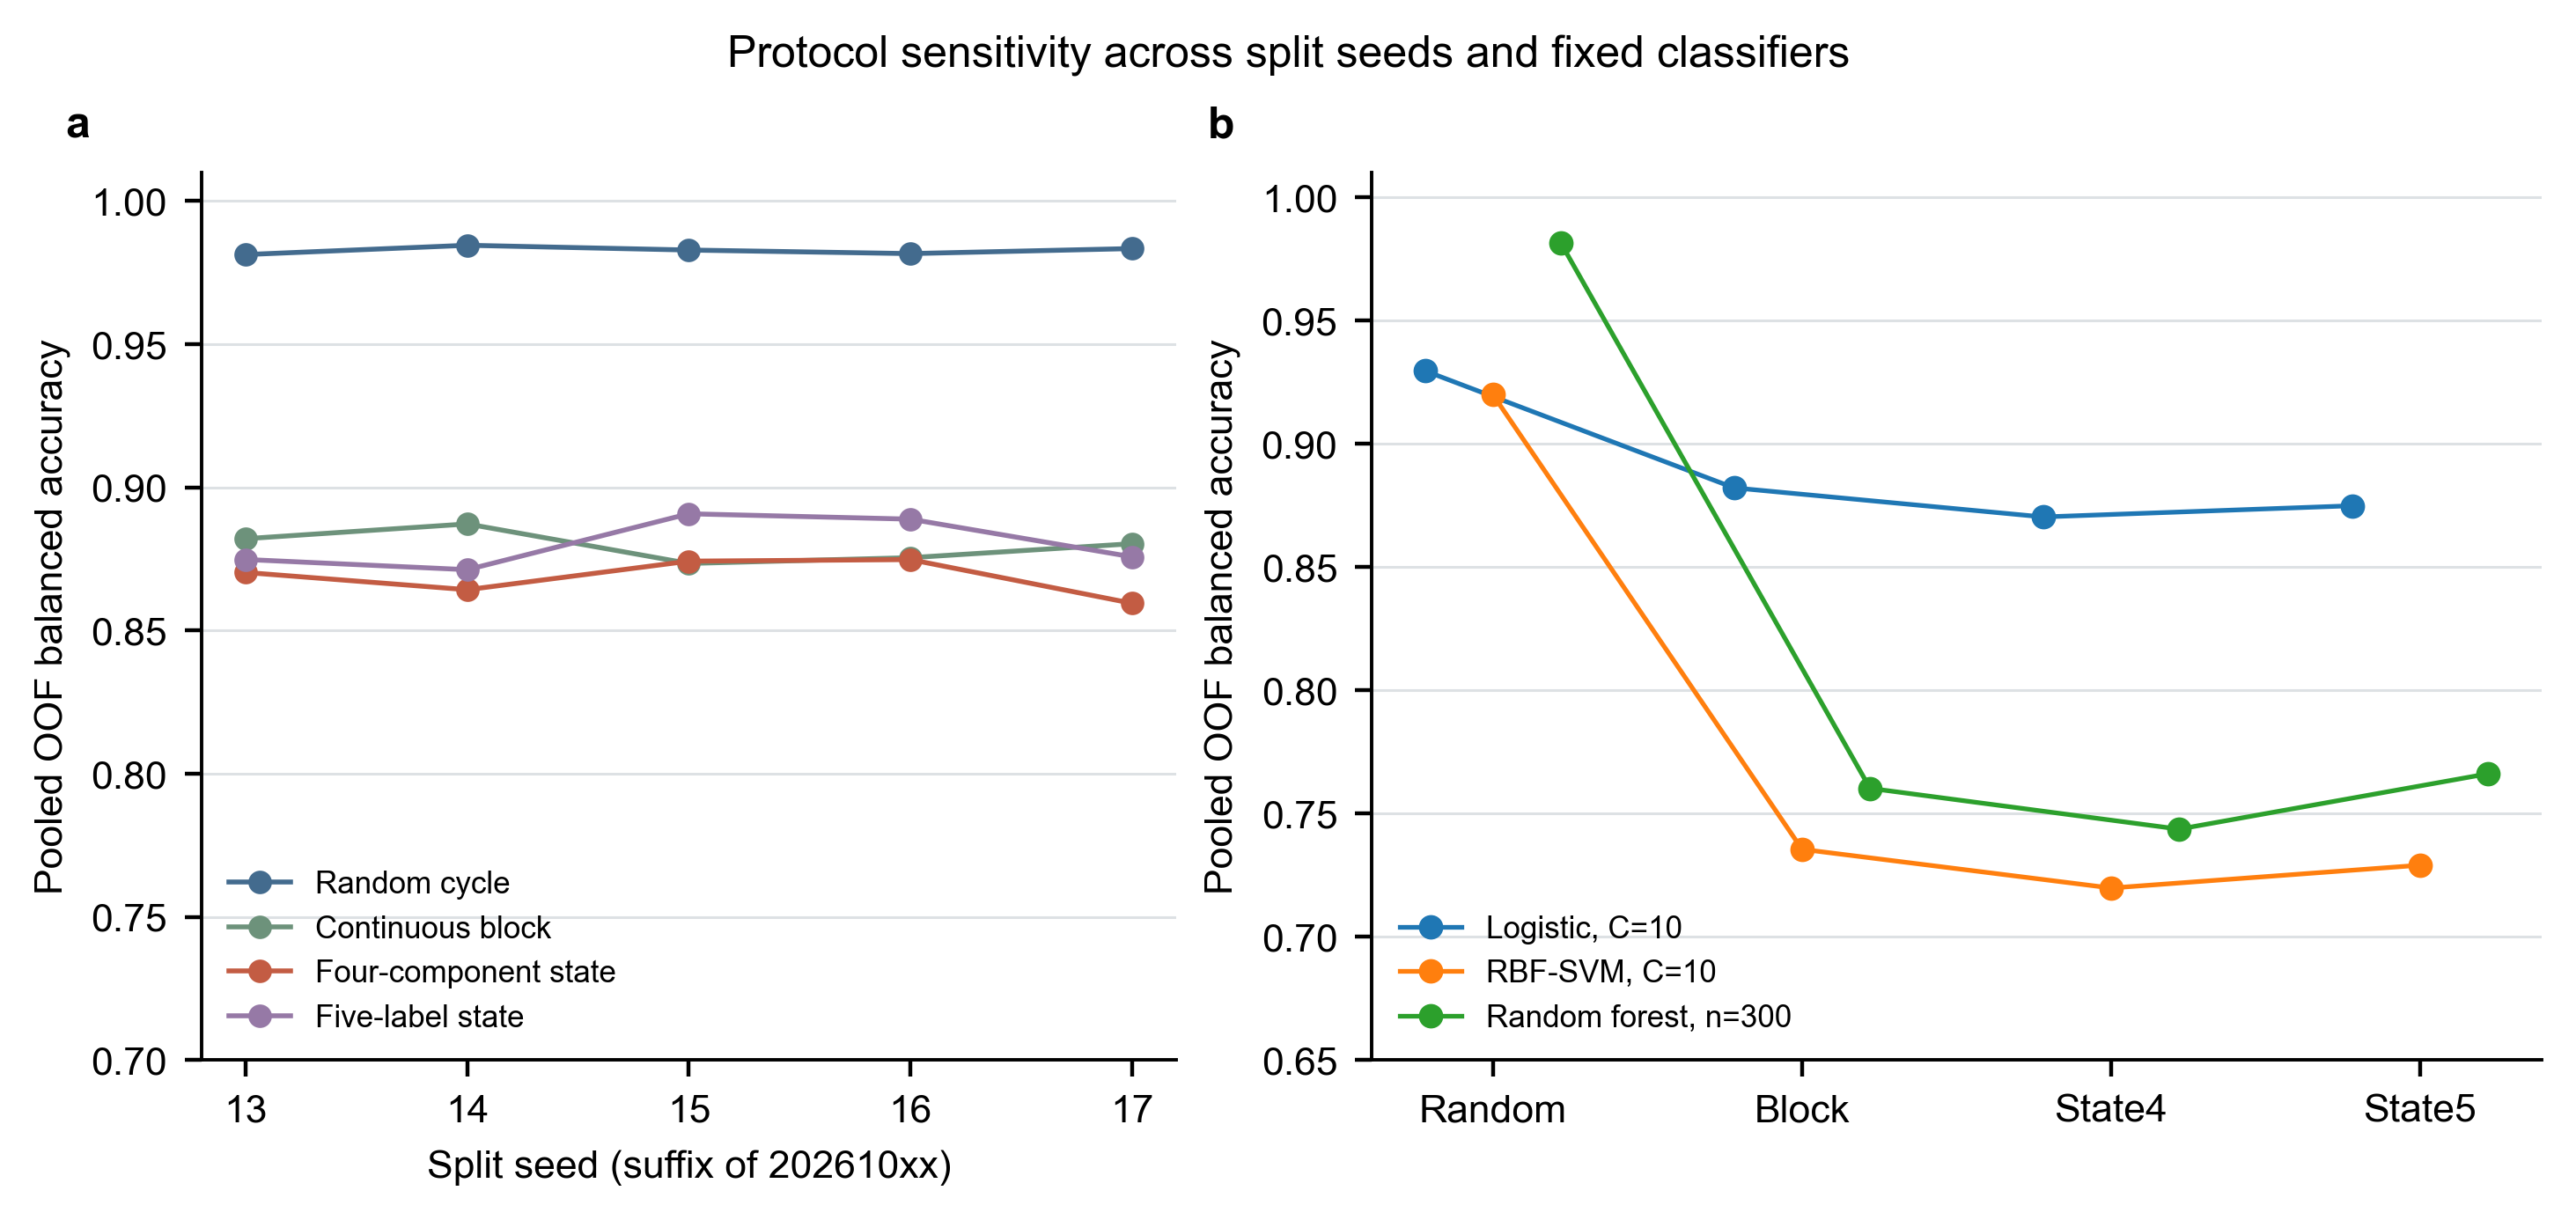
\includegraphics[width=0.98\linewidth]{hydraulic_protocol_robustness_20261013.png}
\caption{Accumulator classification under split seeds and fixed classifiers. Panel (a) shows pooled OOF balanced accuracy for four protocols and five seeds; panel (b) shows pooled OOF balanced accuracy for fixed logistic regression, RBF-SVM, and random forest under the four protocols. The five seeds reuse the same cycles and are not independent experimental repetitions; the plot does not show confidence intervals or significance.}
\label{fig:protocol}
\end{figure}

\subsection{Accumulator classification under the main protocol}

For the \code{pressure\_power}, state4-OC, seed-20261013 reference run, accumulator pooled OOF balanced accuracy is 0.870, macro F1 is 0.866, and accuracy is 0.884. Majority voting over the 144 four-component combinations gives group-level accuracy 0.938. All five outer folds select logistic regression with $C=10$. The cycle-level confusion matrix is shown in Table~\ref{tab:confusion}; the five-seed median and range have already been reported in Table~\ref{tab:main}.

\begin{table}[htbp]
\centering\small
\caption{Cycle-level state4-OC confusion matrix for accumulator pressure levels (seed 20261013). Rows are true labels and columns are predictions, in bar.}
\label{tab:confusion}
\begin{tabular}{lrrrr}
\toprule
True $\backslash$ predicted & 90 & 100 & 115 & 130\\
\midrule
90 & 758 & 30 & 15 & 5\\
100 & 21 & 334 & 44 & 0\\
115 & 1 & 37 & 329 & 32\\
130 & 4 & 4 & 63 & 528\\
\bottomrule
\end{tabular}
\end{table}

Of 256 classification errors, 227 are adjacent-level errors and 29 span at least two level indices. Of the 50 errors in the 90-bar class, 20 are assigned to 115 or 130~bar. Errors are therefore concentrated in adjacent levels but include non-adjacent confusion.

\subsection{Paired error comparison between discrete classification and numeric regression}

In the post hoc descriptive pairing on the same state4-OC OOF cycles, mapping classifier predictions to nominal bar values yields MAE 1.83~bar, RMSE 5.74~bar, $R^2=0.878$, exact-level accuracy 0.884, one-neighbour hit rate 0.987, and mean level distance 0.133 over 2,205 cycles. Raw numeric regression yields MAE 7.74~bar, RMSE 11.85~bar, $R^2=0.480$, nearest-level accuracy 0.689, one-neighbour hit rate 0.906, and mean level distance 0.446. The two OOF tables match cycle ID, true label, and outer fold one by one. In each outer fold, a majority-class baseline predicts the most frequent training label and a mean baseline predicts the training-fold mean; neither uses test-fold features or labels.

Regression outputs are below 90 or above 130~bar for 352/2,205 cycles (16.0\%), with a prediction range of 64.82--198.50~bar. After mapping to the nearest level, counts at distances 0, 1, 2, and 3 are 1,519, 478, 119, and 89. Of the 208 errors spanning at least two levels, 200 arise in outer fold 2. That fold contains 21.6\% of the cycles but contributes 41.7\% of the absolute error and 65.2\% of the squared error; its MAE is 14.94~bar and $R^2=-0.731$, and it selects RBF-SVR with $C=100$. Its inner mean MAE is 5.68~bar, while its outer-fold performance is much worse. Out-of-range predictions and severe level errors are distinct diagnostics: the former has 352 cases, whereas the latter is concentrated in fold 2. A cycle-level cross-tabulation found no overlap between the two events, so they are not a single ``primary'' error type. We did not preregister or statistically test a ranking between them. The fold diagnostic indicates fold-mismatch risk; it does not justify deleting the fold or identify a single cause. A read-only composition check further showed that fold 2 contains a 200-cycle long block (block 64), representing 42.0\% of its 476 cycles. The block corresponds to profile \texttt{20\_100\_0\_90}, stable=1, and true 90~bar; its regression MAE is 31.10~bar and its mean prediction is 121.10~bar. This localizes a candidate mechanism involving fold composition and unequal block sizes while leaving feature-distribution and model-mismatch explanations open.

To reduce confusion from different output spaces and objectives, the fairness audit used the identical state4-OC outer folds, 70 features, and training-only preprocessing for clipped regression, a cumulative-threshold ordinal control, majority/mean baselines, and matched linear/RBF/random-forest families. Raw regression MAE was 7.741~bar and became 6.666~bar after clipping predictions to 90--130~bar; the ordinal control had MAE 2.433~bar and balanced accuracy 0.830, while the classification mapping had MAE 1.828~bar. The majority baseline had accuracy 0.366, balanced accuracy 0.250, and mapped MAE 17.200~bar; the mean baseline had MAE 15.394~bar, RMSE 16.696~bar, and $R^2=-0.032$. Within the fixed linear family, classification mapping MAE was 1.828~bar and clipped-regression MAE was 5.018~bar. These results support a protocol-specific descriptive difference for four discrete nominal levels, not universal classification superiority or continuous-pressure measurement. Details are in the fair-comparison audit record.

\begin{figure}[htbp]
\centering
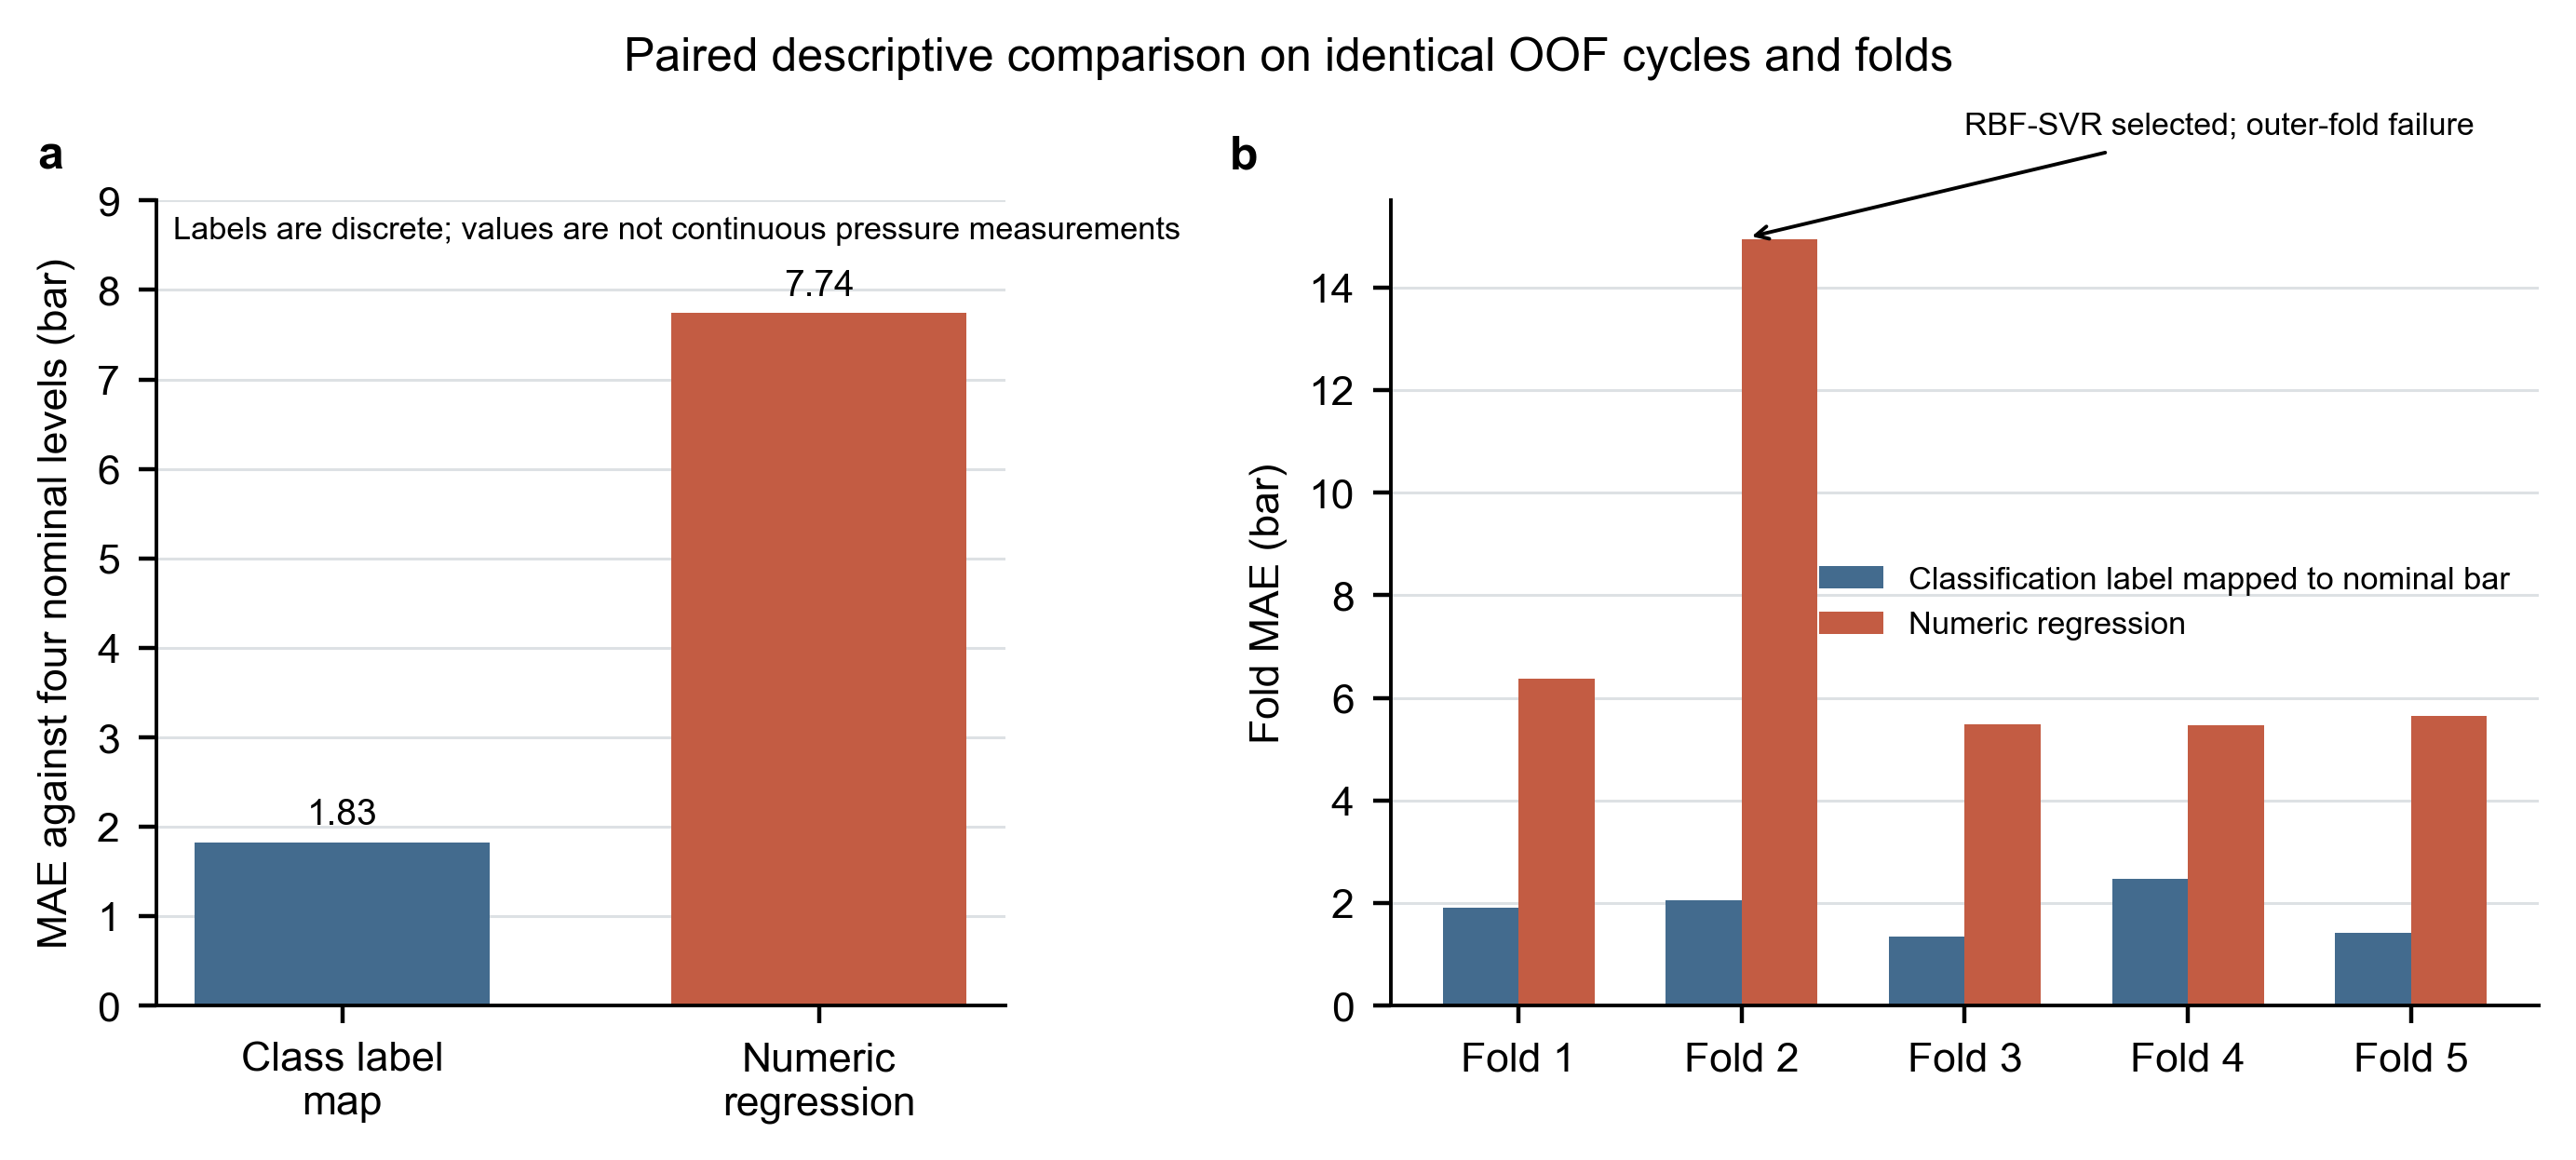
\includegraphics[width=0.98\linewidth]{hydraulic_estimator_comparison_20261013.png}
\caption{Descriptive pressure-error comparison on the same state4-OC OOF cycles. Panel (a) compares pooled OOF MAE for classification predictions mapped to nominal levels and numeric regression; panel (b) shows MAE by outer fold. The mapped classifier output consists of four discrete nominal values and is not continuous-pressure measurement. The higher regression error in fold 2 does not justify dropping the fold or assigning a single cause.}
\label{fig:estimators}
\end{figure}

The lower mapped-classification error does not mean that the classifier measures arbitrary continuous pressure. The labels contain four set points, the classifier is optimized by balanced accuracy, and the mapping has no between-level resolution. The comparison only indicates that, for the present discrete-label task, continuous regression did not yield lower nominal-level error. Regression is retained as an auxiliary analysis to show raw output range and fold instability.

\subsection{Supplementary classification and conditional stratification}

To address the fact that the state4-OC grouping key contains the target label, we also ran a supplementary $context3=\texttt{cooler}\times\texttt{valve}\times\texttt{pump\_leak}$ grouping. With fixed logistic regression ($C=10$), training-only scaling, and seed 20261013, all 36 context3 combinations were isolated from their training folds and each retained all four accumulator levels. Pooled balanced accuracy was 0.894, context-equal balanced accuracy was 0.892, and the minimum context balanced accuracy was 0.675. This post hoc same-rig sensitivity analysis is a more direct non-target-context comparison, but it is not independent-equipment or batch validation.

The supplementary pump-leakage state4-OC classification has pooled OOF balanced accuracy 0.985 and macro F1 0.983 in the original seed. This is a descriptive result for observed component combinations on one test rig. For seed 20261013, accumulator state4-OC balanced accuracy for the five prespecified signal groups is 0.878 for \code{pressure\_flow}, 0.870 for \code{pressure\_power}, 0.835 for \code{all}, 0.820 for \code{physical}, and 0.803 for \code{low\_rate}. \code{physical} is a 14-channel proxy group excluding CE, CP, and SE. This ordering is exploratory. The group comparison has no measurements of installation, calibration, synchronization, maintenance, or bill-of-materials cost, so it is not evidence of a robust channel-group or hardware-cost optimum and is not a new sensor-selection algorithm.

Stratifying the complete main OOF table by stable gives accumulator balanced accuracy 0.881 and macro F1 0.881 for stable=0 (1,449 cycles), versus 0.819 and 0.748 for stable=1 (756 cycles). Stable=1 accumulator-level counts are 439/39/39/239 for 90/100/115/130~bar. Among the 36 state4-OC combinations containing both stable values, stable=0 has 369 cycles with counts 99/90/90/90, while stable=1 has 756 cycles with the same 439/39/39/239 composition. Those 756 stable=1 cycles are the same cycles as the complete stable=1 stratum, rather than a newly sampled common-support subset. In this common-support subset, balanced accuracy is 0.856 for stable=0 and 0.819 for stable=1, a difference of 0.037, approximately 40\% smaller than the full-stratum difference. The strata differ in sample size and label composition, and no state-combination-weighted paired estimate is made; these values are conditional descriptions, not causal effects of stable status. Overall, stable=0, and stable=1 pump-leakage balanced accuracy is 0.985, 0.988, and 0.967, respectively.

\section{Discussion}
\subsection{The split protocol changes the estimand}
Across five seeds, random-cycle splitting gives a higher accumulator point estimate than state4-OC, while the weighting audit gives different summaries when cycles, observed combinations, or profile blocks are weighted equally. The protocol changes test composition, shared operating-condition information, and the model-selection environment at the same time. The random--state4-OC difference is therefore a property of the full evaluation workflow. It is consistent with similar cycles crossing folds under random evaluation, but the data do not identify a separate causal leakage amount.

State4-OC prevents an identical four-component combination from crossing an outer fold while retaining the pressure levels in other combinations. It approximates identification of observed pressure levels under an unseen observed combination. Profile-contiguous blocks and state5 represent profile-derived adjacent segments and combinations including the stable flag; neither is an equipment or batch identifier. The prediction or deployment unit should be defined before choosing the grouping rule.

\subsection{Target representation determines the pressure-error interpretation}
The accumulator labels contain four nominal pressure settings. Mapping classification labels to nominal pressure values measures the error of discrete level identification, whereas numeric regression allows between-level outputs and carries a continuous-value interpretation. In the present discrete task and state4-OC workflow, the mapped classification output has lower nominal-pressure error than regression. This is not a general ranking of continuous-pressure algorithms. A continuous-pressure study would require continuous reference measurements, more settings, and independent acquisition batches.

\subsection{Relation to prior work and evaluation increment}
The study shares the UCI data context with prior multi-component classification, sensor-attribution, and blockwise conformal work, but addresses a different question. It registers and compares four split protocols under nested model selection and multi-seed OOF evaluation, and places discrete-level errors, regression out-of-range predictions, and weighting sensitivity in one audit framework. The high accuracy reported by Zhan and Liu~\cite{zhan} motivates the audit rather than serving as a same-target benchmark; the preprint~\cite{bui} covers part of the grouping question and provides blockwise joint conformal coverage guarantees, whereas this study provides neither conformal intervals nor coverage guarantees and does not reproduce its numerical results. The contribution is therefore framed as a dataset-level evaluation supplement. The transparency assessment of this direct neighbor is page-grounded: page 2 describes preprocessing and task construction but does not provide a reproducible train/test proportion, split unit, random seed, or test-set composition; on page 4, Figure 3 labels 20 particles and 30 iterations while the prose uses the reverse wording. This concerns report reproducibility and does not invalidate the reported result.

\subsection{Limitations and practical implication}
The evidence has three boundaries: all results come from one public rig without independent equipment, acquisition-batch, or calibration identifiers; the five seeds reuse the same cycles and were added after inspection of the initial result, so they are sensitivity descriptions rather than independent confirmation; and the main analysis uses fixed summary features and a limited candidate grid, while channel-group results contain no hardware-cost or deployment measurements. The supported practical output is a dataset-level reporting recommendation: state the split and its estimand, and report cycle-weighted, group-weighted, and discrete-level errors when those quantities answer different questions. External data with equipment or batch identifiers are needed for external validation.

\section{Conclusion}
On the public hydraulic test-rig dataset, the split protocol changes both the accumulator classification point estimate and the estimand. Across five seeds, random-cycle pooled OOF balanced accuracy is 0.981--0.985, compared with 0.860--0.875 for state4-OC. Cycle-, state4-combination-, and profile-block-weighted classification accuracies are 0.884, 0.876, and 0.866, respectively; corresponding regression MAE values are 7.74, 5.35, and 5.39~bar. These differences belong to the full evaluation workflow and are not an identified causal leakage amount.

The four nominal pressure levels support discrete state identification and nominal-level error auditing, but provide no evidence for continuous-pressure or cross-device performance. The limited increment is a reproducible framework that links split protocol, estimand, weighting, and error representation for application evaluation on public hydraulic data.

\section*{Data and research statements}

\textbf{Data availability.} The raw data are public through the UCI Machine Learning Repository, with DOI 10.24432/C5CW21 and CC BY 4.0 licence. The data files, derived features, and OOF results used here are stored in the research project package; the local reproducibility manifest records file sizes and SHA-256 hashes at \texttt{results/reproducibility\_manifest\_20261016.json}. The project has not yet created a public permanent archive or DOI; code and derived-data release must be completed before submission.

\textbf{Code availability.} Cleaning, feature extraction, cross-validation, metric recomputation, and plotting scripts are in the \code{src/} directory of the accompanying research package, with the entry point \texttt{scripts/reproduce\_hydraulic\_audit.ps1}. No public code repository or permanent archive has been created at the time of finalizing this manuscript; actual links must be added after publication.

\textbf{Ethics statement.} This study analyses only public equipment-operation signals from the UCI repository and involves no human participants, personal data, or animal experiments; no ethics approval process was undertaken. If the target journal or the author's institution requires a formal exemption determination for secondary analysis of public data, the author should complete that determination before submission.

\textbf{Funding and conflicts of interest.} No external funding was received. The author declares no competing interests.

\textbf{Author contributions.} Chen-Yu Yan completed the conceptualization, data curation, analysis, manuscript preparation and review.

\textbf{Preregistration.} No verifiable preregistration record was found. The five-seed analysis, fixed-model comparison, and paired mapping from classification predictions to nominal bar values should be understood as post-audit supplementary or derived analyses.

\begin{thebibliography}{15}
\bibitem{uci} UCI Machine Learning Repository. Condition monitoring of hydraulic systems. Dataset. DOI: \href{https://doi.org/10.24432/C5CW21}{10.24432/C5CW21}. \url{https://archive.ics.uci.edu/dataset/447/condition+monitoring+of+hydraulic+systems}.

\bibitem{helwigstats} Helwig N, Pignanelli E, Sch{\"u}tze A. Condition Monitoring of a Complex Hydraulic System Using Multivariate Statistics. In: \emph{2015 IEEE International Instrumentation and Measurement Technology Conference (I2MTC)}; 2015. DOI: \href{https://doi.org/10.1109/I2MTC.2015.7151267}{10.1109/I2MTC.2015.7151267}.

\bibitem{helwigfault} Helwig N, Pignanelli E, Sch{\"u}tze A. Detecting and Compensating Sensor Faults in a Hydraulic Condition Monitoring System. \emph{SENSOR 2015}. 2015:641--646. DOI: \href{https://doi.org/10.5162/sensor2015/D8.1}{10.5162/sensor2015/D8.1}.

\bibitem{schneider} Schneider T, Helwig N, Sch{\"u}tze A. Automatic feature extraction and selection for classification of cyclical time series data. \emph{tm -- Technisches Messen}. 2017;84(3):198--206. DOI: \href{https://doi.org/10.1515/teme-2016-0072}{10.1515/teme-2016-0072}.

\bibitem{yildirim} Yildirim C, Franco-Pereira AM, Lillo RE. Condition monitoring and multi-fault classification of hydraulic systems using multivariate functional data analysis. \emph{Heliyon}. 2025;11(1):e41251. DOI: \href{https://doi.org/10.1016/j.heliyon.2024.e41251}{10.1016/j.heliyon.2024.e41251}.

\bibitem{konig} K{\"o}nig C, Helmi AM. Sensitivity Analysis of Sensors in a Hydraulic Condition Monitoring System Using CNN Models. \emph{Sensors}. 2020;20(11):3307. DOI: \href{https://doi.org/10.3390/s20113307}{10.3390/s20113307}.

\bibitem{bui} B{\`u}i Thanh L{\^a}m. Blockwise Joint Conformal Prediction for Simultaneous Multi-Component Condition Monitoring of Hydraulic Systems. EngrXiv preprint, 2026-08-10. DOI: \href{https://doi.org/10.31224/7905}{10.31224/7905}.

\bibitem{askari} Askari B, Carli R, Cavone G, Dotoli M. Data-Driven Fault Diagnosis in a Complex Hydraulic System based on Early Classification. \emph{IFAC-PapersOnLine}. 2022;55(40):187--192. DOI: \href{https://doi.org/10.1016/j.ifacol.2023.01.070}{10.1016/j.ifacol.2023.01.070}.

\bibitem{roberts} Roberts DR, Bahn V, Ciuti S, et al. Cross-validation strategies for data with temporal, spatial, hierarchical, or phylogenetic structure. \emph{Ecography}. 2017;40(8):913--929. DOI: \href{https://doi.org/10.1111/ecog.02881}{10.1111/ecog.02881}.

\bibitem{varma} Varma S, Simon R. Bias in error estimation when using cross-validation for model selection. \emph{BMC Bioinformatics}. 2006;7:91. DOI: \href{https://doi.org/10.1186/1471-2105-7-91}{10.1186/1471-2105-7-91}.

\bibitem{zhou} Zhou Rusheng, Jiao Zongxia, Wang Shaoping. Research status and development trends of hydraulic-system fault-diagnosis technology. \emph{Journal of Mechanical Engineering}. 2006;42(09):6--14. DOI: \href{https://doi.org/10.3901/JME.2006.09.006}{10.3901/JME.2006.09.006}. [Chinese article.]

\bibitem{zhaoxu} Zhao Xiuxu, Zhou Chuanli, Hu Zhehao, et al. Experimental study of multi-component fault-mode identification in hydraulic systems. \emph{Hydraulics and Pneumatics}. 2014(06):34--38. DOI: \href{https://doi.org/10.11832/j.issn.1000-4858.2014.06.009}{10.11832/j.issn.1000-4858.2014.06.009}. [Chinese article.]

\bibitem{shan} Shan Zenghai, Li Zhiyuan, Zhang Xu, et al. Health-state assessment of hydraulic pumps based on multisensor information fusion and a multi-granularity cascade forest model. \emph{China Mechanical Engineering}. 2021;32(19):2374--2382. DOI: \href{https://doi.org/10.3969/j.issn.1004-132X.2021.19.013}{10.3969/j.issn.1004-132X.2021.19.013}. [Chinese article.]

\bibitem{zheng} Zheng Biao, Gao Bingpeng, Cheng Jing. Fault-severity diagnosis of hydraulic pumps based on DNN-CapsNet. \emph{Hydraulics and Pneumatics}. 2023;47(08):41--49. DOI: \href{https://doi.org/10.11832/j.issn.1000-4858.2023.08.006}{10.11832/j.issn.1000-4858.2023.08.006}. [Chinese article.]

\bibitem{zhan} Zhan Xin, Liu Zhuoya. Hydraulic-system fault-diagnosis model based on the PSO-SES-BPNN algorithm. \emph{Journal of Ordnance Equipment Engineering}. 2023;44(04):172--178. DOI: \href{https://doi.org/10.11809/bqzbgcxb2023.04.024}{10.11809/bqzbgcxb2023.04.024}.
\end{thebibliography}

\end{document}
